\documentclass{ufsc-thesis}

% Gerador de texto
\usepackage{lipsum}

\usepackage{cmap}
\usepackage[utf8]{inputenc}
\usepackage[T1]{fontenc}
\usepackage{geometry}
\usepackage{graphicx}
\usepackage{float}
\usepackage{algorithm}
\usepackage[noend]{algpseudocode}
%\usepackage[pdftex]{graphicx}
%\usepackage{graphviz}

% Preâmbulo
\titulo{ParaQuantumSAT: Um algoritmo \textit{SAT solver} distribuído}
\autor{João Guilherme Zeni}
\data{\today}
\instituicao{Universidade Federal de Santa Catarina}
\local{Florianópolis, SC-Brasil}
\tipotrabalho{Trabalho de Conclusão de Curso}
\orientador{Jerusa Marchi}
\coorientador{Mario Dantas}
\programa{Graduação em Ciências da Computação}
% \preambulo{Modelo can\^{o}nico de trabalho de conclusão de curso para acadêmicos da UFSC e usuários da plataforma \abnTeX.}
\centro{Centro Tecnológico -- CTC}
\assuntos{Algoritmos, Computação Paralela}

\begin{document}
% Inicia parte pré-textual do documento capa, folha de rosto, folha de
% aprovação, aprovação, resumo, lista de tabelas, lista de figuras, etc.
\pretextual%
\imprimircapa%
\imprimirfolhaderosto*%
\clearpage
%\imprimirfichacatalografica%
\tableofcontents%


\chapter{Resumo}

Computação paralela é uma área de estudo crítica, visto que hoje
a capacidade de processamento dos computadores cresce com a paralelização dos processadores. Um
dos principais desafios em computação paralela é a construção de 
algoritmos paralelos eficientes para resolver problemas clássicos 
de computação. Este trabalho se propõe a desenvolver um algoritmo 
\textit{SAT solver} paralelo, tendo como base um algoritmo SAT solver sequencial.

Palavras Chave :Algoritmos Paralelos, \textit{SAT Solver}


\chapter{Introdução}
\label{cap:introduction}

Originalmente a computação paralela era um campo de estudo apenas 
utilizado em computação científica, dada a grande demanda por poder 
computacional desta área. Hoje porém computação paralela está sendo 
utilizada em novos cenários, o que tem motivado o crescente estudo de 
algoritmos paralelos. Um desses cenários é o de Redes de Sensores sem Fio, 
pois estas funcionam como diversos dispositivos que se 
comunicam. Outro cenário é o de processadores multi-core que se 
tornaram populares desde que foi atingida a barreira de potência, 
que fez com que não seja mais possível aumentar a potência de um 
processador individualmente\cite{patterson2012computer}.

O problema da satisfazibilidade booleana(SAT)\cite{Biere} consiste em determinar, 
para uma dada fórmula booleana, se existe uma atribuição de valores 
para as variáveis para a qual a fórmula é satisfeita. SAT é um problema 
NP-Completo, logo sua resolução por si só é um dos maiores problemas da 
computação. Porém o SAT tem aplicações diretas em outras áreas da 
computação como verificação formal e inteligência artificial, 
tornando-o um problema interessante para o uso e estudo de 
computação paralela.

Computação paralela\cite{Kumar2002} começou a despertar o interesse dos pesquisadores 
de algoritmos \textit{SAT solvers} quando foi alcançada a barreira de potência, 
pois estes a consideravam uma boa técnica para resolver o problema de 
forma rápida. 

A principal abordagem ao problema tem sido aplicar técnicas de paralelismo, 
como dividir-e-conquistar, em algoritmos de \textit{SAT solving} consolidadas, 
como DPLL. Porém essa abordagem apresenta alguns problemas, como a 
necessidade de adicionar mecanismos de controle de carga aos algoritmos. 
Neste trabalho usa-se outra abordagem ao problema, a qual usa um algoritmo 
\textit{SAT solver} como base para o desenvolvimento de um novo algoritmos paralelo.


\section{Objetivos}
\label{sec:objets}

O presente trabalho tem por objetivo geral o desenvolvimento de um 
algoritmo \textit{SAT solver} paralelo, tendo como base um algoritmo sequencial.

\subsection{Objetivos Específicos}

Os objetivos específicos deste trabalho estão listados abaixo:

\begin{enumerate}
  \item Compreender as técnicas de computação paralela e quais são mais adequadas para se utilizar no algoritmo \textit{SAT solver}.
  \item Compreender a abordagem utilizada no algoritmo \textit{SAT solver} QuantumSAT.
  \item Desenvolver o algoritmo \textit{SAT solver} paralelo.
  \item Testar o algoritmo desenvolvido, usando teorias SAT aleatórias.
  \item Comparar os resultados do algoritmo desenvolvido com outros já existentes.
  \item Submeter o algoritmo a uma competição, visando sua avaliação definitiva.
  \item Redação do TCC e dos artigos técnicos.
\end{enumerate}

\section{Justificativa}
\label{sec:just}

O SAT é um problema que apresenta diversas aplicações na indústria
atual, além disso ele também possui grande importância teórica 
na ciência da computação.

A computação paralela sempre possuiu grande importância quando 
se trata de aplicações científicas ou de grande volumes de 
dados/processamento, porém a partir do momento que atingiu-se 
a barreira de potência a área tem ganhado importância em todas as 
áreas da computação, dado que processadores multi-core hoje são 
os mais usados.

Logo a pesquisa de algoritmos \textit{SAT solvers} paralelos se justifica na 
intersecção entre as justificativas para a pesquisa nessas duas áreas,
dado que hoje todas as áreas que utilizando \textit{SAT solver} tem como ferramenta 
de trabalho processadores multi-core e necessitam de algoritmos que 
funcionem de forma eficiente nesses processadores.

\chapter{Fundamentação Teórica}
\label{chap:fund}

Neste capítulo são descritos os fundamentos necessários para a
compreensão do trabalho desenvolvido.

\section{O problema SAT}
\label{sec:sat}

Para o compreensão do problema SAT é necessária a compreensão 
de algumas definições básicas de lógica, apresentadas a seguir.

Proposição é uma sentença a qual pode ser atribuído um sentido, 
chamado de asserção. Uma proposições podem ser simples ou compostas. Neste 
trabalho utilizaremos proposições lógicas, cujas asserções são 
Verdadeiro ou Falso. Proposições lógicas simples correspondem a 
variáveis. Proposições complexas são 
proposições simples conectadas por operadores lógicos. Quando 
existem variáveis sem valor atribuído uma proposição chama-se 
de fórmula proposicional, representada neste trabalho por $\Phi$.

Fórmulas proposicionais são escritas utilizando operadores lógicos,
que são símbolo utilizado para se trabalhar com sentenças lógicas. 
Estes operadores possuem caráter binário, sendo usados para conectar 
duas sentenças lógicas, e caráter unário, para atribuir uma propriedade 
a uma sentença lógica. Para este trabalho notam-se os operadores 
\textit{AND} representado por $\wedge$, \textit{OR} representado 
por $\vee$ e \textit{NOT} representado por $\neg$. As interpretações 
destes operadores são descritos na tabela \ref{tab:a}.

%\nomenclature{$\wegde$}{Representação do AND lógico.}
%\nomenclature{$\vee$}{Representação do OR lógico.}
%\nomenclature{$\neg$}{Representação do NOT lógico.}

\begin{table}[H]
\begin{center}
\begin{tabular}{@{}|l|l|l|l|l|@{}}
\toprule
\multicolumn{2}{|l|}{\textbf{Entradas}} & \multicolumn{3}{l|}{\textbf{Saídas}} \\ \midrule
A                  & B                  & A $\wedge$ B         & A $\vee$  B         & $\neg$A        \\ \midrule
V                  & V                  & V           & V           & F        \\ \midrule
V                  & F                  & F           & V           & F        \\ \midrule
F                  & V                  & F           & V           & V        \\ \midrule
F                  & F                  & F           & F           & V        \\ \bottomrule
\end{tabular}
\caption{Tabela lógica}\label{tab:a}
\end{center}
\end{table}

Fórmulas proposicionais podem ser representadas de diversas formas, porém 
toda fórmula proposicional pode ser representa nas duas formas 
canônicas, a forma normal conjuntiva(CNF, sigla em inglês) e a 
forma normal disjuntiva(DNF, sigla em inglês).

As fórmulas proposicionais em CNF são representadas como uma 
conjunção de cláusulas, sendo cada cláusula uma disjunção de literais, 
onde cada literal pode assumir Verdade ou Falso, 
como é apresentado abaixo na equação \ref{eq:CNF}. Toda fórmula proposicional pode ser 
convertida para forma CNF através de um procedimento trivial. 
O padrão de entrada da grande maioria dos \textit{SAT solvers} é o Dimacs, 
que representa fórmulas proposicionais na forma CNF.

\begin{equation} \label{eq:CNF}
F = C_1\wedge C_2\wedge C_3 \dots \wedge C_k\ |\ \forall C, C_n = L_1\vee L_2 \vee L_3 \dots \vee L_k
\end{equation}

As fórmulas proposicionais em DNF são representadas como uma 
disjunção de cláusulas, sendo cada cláusula um conjunção de literais, 
como é apresentado abaixo na equação \ref{eq:DNF}. A conversão de uma fórmula proposicional 
para forma DNF é por si só uma solução para o problema, portanto 
uma tarefa NP-Completa. Para realizar esta conversão existem 
diversas técnicas, neste trabalho será apresentada em detalhes 
uma delas.

\begin{equation} \label{eq:DNF}
F = D_1\vee D_2\vee D_3 \dots \vee D_k\ |\ \forall D, D_n = L_1\wedge L_2 \wedge L_3 \dots \wedge L_k
\end{equation}

O problema SAT é definido sobre uma linguagem de lógica proposicional $\mathcal{L}(P)$, 
onde P = {$p_1,p_2,\dots,p_n$} sendo que todo p é um símbolo proposicional sem 
valor verdade definido. Uma fórmula $\Phi \in$ L(P) pode ser escrita em CNF, 
logo $\Phi = \{C_1\wedge C_2 \dots \wedge C_k | \forall C, C_n = p_i \vee \neg p_j \dots \vee p_z\}$.
Com isto pode-se definir o problema SAT como sendo responder se existe um 
conjunto de atribuição de valores verdade a P, o qual faz com que $\Phi$ 
seja verdade, caso exista esse conjunto $\Phi$ é dito satisfazível. O exemplo 
abaixo apresenta um problema SAT.

Seja $\Phi$:

$$0: (\neg p_4\vee p_2 \vee\neg p_3) \wedge $$
$$1: (\neg p_3\vee p_2 \vee\neg p_1) \wedge $$
$$2: ( p_5\vee\neg p_2 \vee\neg p_3) \wedge $$
$$3: (\neg p_2\vee p_5 \vee\neg p_1) \wedge $$
$$4: (\neg p_3\vee p_5 \vee p_1) \wedge $$
$$5: ( p_4\vee p_5 \vee p_2) \wedge $$
$$6: (\neg p_5\vee p_3 \vee\neg p_2) \wedge $$
$$7: (\neg p_1\vee p_4 \vee p_3) \wedge $$
$$8: (\neg p_3\vee\neg p_2 \vee\neg p_1) \wedge $$
$$9: (\neg p_3\vee\neg p_4 \vee\neg p_1) $$

Assim podemos ver que se $\neg p_2$ for Verdade então as cláusulas
2, 3, 6 e 8 serão Verdade, se $\neg p_3$ for Verdade então as cláusulas 
0, 1, 4 e 9 serão Verdade e se $p_4$ for Verdade então as cláusulas 
5 e 7 serão Verdade, como foi possível atribuir valores que fizeram com 
que todas as cláusulas de $\Phi$ sejam Verdade disse-se que $\Phi$ é satisfazível.

Outra característica do problema SAT é número de símbolos em cada cláusula,
o problema usualmente é chamado de $k$SAT onde $k$ é número de símbolos em cada 
cláusula, no caso anterior o problema é um 3SAT. Esta característica 
é importante pois toda fórmula proposicional pode ser escrito como um 3SAT. 
Outro fato importante é o de que os problemas que podem ser escritos em 
2SAT possuem complexidade O(n), porém não é garantido que todas as fórmulas proposicionais 
possam ser escritas na forma 2SAT\cite{Biere}.

\section{Importância do Problema SAT}
\label{sec:ipsat}

A resolução de problemas SAT possui aplicação direta em diversas áreas, 
nesta seção serão apresentadas algumas delas e como SAT é utilizado nestas 
aplicações.

O projeto de sistemas digitais é amplamente auxiliado pelas mais diversas 
ferramentas, muitas delas se utilizam de \textit{SAT solvers}\cite{Lavagno2006}. Uma delas é verificação 
de equivalência, que consiste em verificar se para dois circuitos digitais 
distintos com o mesmo conjunto de entradas o conjunto de saídas será igual, 
para se resolver este problema as funções de entradas e saídas dos circuitos 
são escritos como uma fórmula proposicional e verifica-se a satisfazibilidade 
com um \textit{SAT solver}.

Uma aplicação bem sucedida da solução de SAT é o \textit{automate planning} em 
inteligência artificial\cite{Kautz1992}. O problema \textit{planning} consistem em, 
dado um conjunto de estados e um conjunto de transições entre estados, 
descobrir se é possível sair de um estado inicial e atingir um estado 
objetivo em um número finito de transições. Uma solução para este problema 
se chama satplan\cite{Kautz1992}, que consiste em converter o problema do \textit{planning}
para uma fórmula proposicional e verificar se a mesma é satisfazível, isto é 
feito de forma iterativa começando do planejamento com 1 passo e indo até 
o limite de passos dado pelo problema.

Outra aplicação da solução SAT importante são os \textit{model checkers}\cite{Biere},
que consistem em dado um modelo automaticamente verificar se este modelo 
atende a dadas especificações. \textit{Model checkers} possuem ampla aplicação, 
principalmente em teste de sistemas, que vão de hardware a protocolos de comunicação.
Este problema apresenta uma solução similar a do \textit{planning}, pois sua solução 
consiste em converter o modelo em uma fórmula proposicional e a partir dai utilizar um 
\textit{SAT solver}\cite{Clarke2001}. Esta técnica é a mais utilizada nos casos de verificadores 
restritos e quando as especificações são dadas através de fórmulas em lógica 
temporal.

\section{Algoritmos SAT Solvers}
\label{sec:solver}

Os \textit{SAT solvers} podem ser divididos em classes, sendo que as 
duas principais classes de algoritmos \textit{SAT solvers} sequenciais 
são os baseados em conflito de cláusulas(CDCL, sigla em inglês), a 
versão mais moderna do DPLL(Davis-Putnam-Logemann-Loveland)\cite{Davis1962}, e os 
baseados em busca local estocástica\cite{Selman95}. O algoritmo \textit{SAT solver} 
desenvolvido neste trabalho é baseado na conversão CNF-DNF, 
não exitem muitos outros \textit{solver} baseados nesse método, 
em \cite{Miltersen} \cite{Katajainen} este método é discutido.

A classe CDCL, e sua versão original o DPLL, são baseados na técnica 
de \textit{backtracking}\cite{Davis1962}. Estes algoritmos consistem em  atribuir um 
valor verdade a uma literal, simplificar a fórmula e, recursivamente, 
verificar se a fórmula simplificada é satisfazível. No caso do DPLL a ideia 
básica é recursivamente montar uma arvore de decisão, como a apresentada na 
figura \ref{fig:DPLL}, além disto são utilizadas diversas heurísticas para melhor eficiência do algoritmo, 
destacam-se aqui as heurísticas para a escolha do literal a se atribuir o 
valor verdade\cite{Ouyang1996}. No caso do CDCL, é montada uma estrutura adicional 
que o permite ignorar alguns passos, para em teorias geradas aleatório 
baixar o tempo médio de execução\cite{Silva1997}. O funcionamento básico do 
CDCL é mostrado na figura \ref{fig:CDCL}.

\begin{figure}[H]
    \centering
    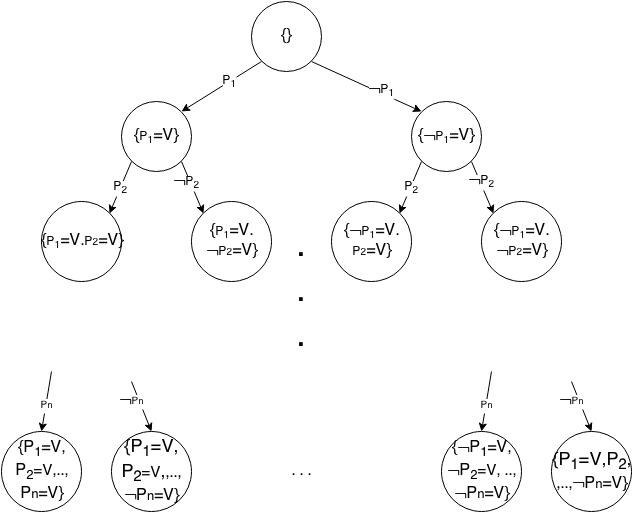
\includegraphics[width=0.6\textwidth]{figuras/DPLL.jpg}
    \caption{Arvore de decisão do DPLL}
    \label{fig:DPLL}
\end{figure}

\begin{figure}[H]
    \centering
    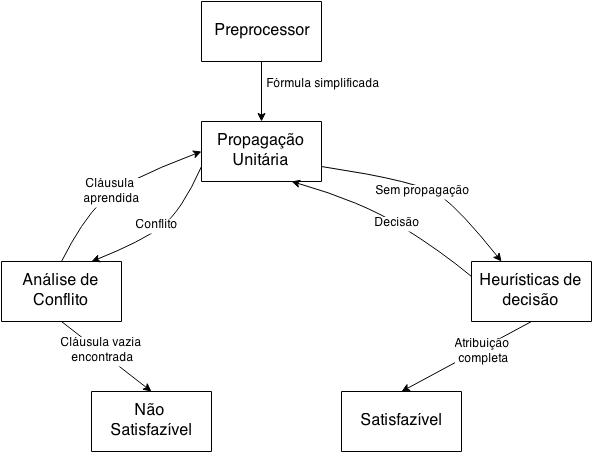
\includegraphics[width=0.6\textwidth]{figuras/CDCL.jpg}
    \caption{Diagrama que apresenta os procedimentos e componentes do CDCL}
    \label{fig:CDCL}
\end{figure}

O algoritmo \ref{alg:DPLL} é o pseudo código de uma versão básica do 
DPLL. Esta versão é bastante simples. O primeiro passo é 
eliminar as cláusulas unitárias, aquelas que contém apenas um literal, 
e as cláusulas que contém o literal da cláusula unitária, pois para a fórmula 
ser satisfazível este literal precisa ser Verdade. O segundo passo é 
eliminar as cláusulas que contém literais puros, aqueles que apresentam apenas 
uma polaridade em toda a fórmula, pois sempre é possível se atribuir Verdade a 
estes símbolos. O terceiro é selecionar aleatoriamente um literal. O quarto 
é executar este algoritmo recursivamente, considerando Verdade para este literal 
e para sua negação.

\begin{algorithm}
\caption{Pseudo código DPLL} \label{alg:DPLL}
\begin{algorithmic}[1]
\Procedure{DPLL}{$\Phi$}
\For{Cláusula unitária $l\ em\ \Phi$}
    \State $\Phi \gets atribui(l,\Phi)$
\EndFor
\For{Literal puro l em $\Phi$}
    \State $\Phi \gets atribui(l,\Phi)$
\EndFor
\State $l \gets escolhaDeLiteral(\Phi)$
\State \textbf{return} $DPLL(\Phi \wedge l) \vee DPLL(\Phi \wedge \neg l)$
\EndProcedure
\end{algorithmic}
\end{algorithm}

Uma implementação do algoritmo CDCL é o \textit{solver} MiniSAT\allowbreak\cite{Een03anextensible}.
Este \textit{solver} implementa várias otimizações que resultam 
em melhorias significativas em casos médios. Vale destacar 
a técnica de minimização de cláusulas conflitantes, pois 
em exemplos indústrias é bastante comum que, mais de 30\% 
dos literais em uma cláusula conflitante, sejam redundantes\cite{MiniSatSystemDesc}.

Já os algoritmos baseados em busca local estocástica consistem em atribuir 
valores verdade a literais de forma iterativa e ir, constantemente, 
melhorando a solução até que a fórmula seja satisfazível\cite{Selman95}. Estes são 
algoritmos gulosos, pois utilizam os literais que eliminam o maior 
número de cláusulas. Possuem diversas formas de otimização, 
por exemplo: aumentar a quantidade de literais a atribuir valor verdade 
em cada passo, implementar métodos para melhor a qualidade da seleção de literais 
de forma iterativa, entre outras. A principal falha deste método 
é sua incompletude, dado que ele é incapaz de afirmar se uma dada 
fórmula proposicional é insatisfazível\cite{Hoos2004}.

O algoritmo \ref{alg:local} é um pseudo código de uma versão básica de um 
algoritmo de busca local estocástica para SAT. O primeiro passo é executar 
um laço para o número de tentativas definido. O segundo é atribuir a todos 
os símbolos um valor verdade aleatório. O terceiro é executar um laço 
para um número de mudanças de símbolos definido. Dentro deste laço 
é verificado se $\Phi$ está satisfeito, caso esteja é retornado $\Phi$. 
Caso não esteja é feita uma mudança aleatória no valor verdade de um símbolo.
Caso não seja encontrada uma solução o algoritmo informa que não foi 
possível encontrar uma solução.

\begin{algorithm}
\caption{Pseudocódigo de um algoritmo de busca local} \label{alg:local}
\begin{algorithmic}[1]
\Procedure{buscaLocal}{$\Phi$}
\For{i := 1 to nTentativas}
    \State{$\Phi \gets$ valoresVerdadeAleatórios($\Phi$)} \Comment{atribui valores verdade
    aleatórios aos literais}
    \For{i := 1 to nMudanças}
        \If{$\Phi$ é satisfeito}
            \State \textbf{return} $\Phi$
        \EndIf
        \State $\Phi \gets mudancaDeLiteral(\Phi)$ \Comment{muda o valor verdade do literal que
        reduzir o maior número de cláusulas}
    \EndFor
\EndFor
\State \textbf{return} Não foi encontrada atribuição satisfazível
\EndProcedure
\end{algorithmic}
\end{algorithm}

Uma implementação desta técnica é o \textit{solver} WalkSAT\cite{Selman95}, 
este \textit{solver} utiliza uma otimização que consiste no modo de escolha 
do literal a alterar o valor verdade, na maioria dos algoritmos 
a escolha é feita de modo a atingir o maior número de cláusulas. No 
WalkSAT está escolha é feita tendo como base quais são as cláusulas que 
estão insatisfeitas. Este \textit{solver} possui um bom resultado 
para fórmulas proposicionais que foram geradas a partir de um problema 
de \textit{planning}, sendo esta sua principal aplicação\cite{Kautz1996}.

Existem outras diversas classes de \textit{SAT solvers} que possuem 
usos específicos. Neste trabalho é utilizado como base um algoritmo 
SAT de uma classe diferente, que é baseada na conversão CNF-DNF. 
Uma vez que a solução de SAT para fórmulas proposicionais em DNF é 
trivial, a conversão é, por si só, uma resolução. Esta técnica é bastante 
antiga sendo sua forma clássica a utilização da lei de De-Morgan para efetuar 
a conversão\cite{Skiena2008}, porém esta solução é extremamente ineficiente\cite{Miltersen2005}. 
Na próxima seção é apresentado o algoritmo base para este trabalho, que 
efetua esta conversão escrevendo a fórmula proposicional na forma DNF 
utilizado uma nova estrutura chamada quantum, que assegura maior eficácia 
ao processo de conversão.

\section{Algoritmo Base}
\label{sec:algbase}

% Utilizar trabalhos da jerusa e outros

Será utilizado como base o algoritmo \textit{SAT solver} QuantumSAT\allowbreak\cite{bittencourt2003syntactic}. 
Este é um algoritmo \textit{SAT solver} completo, cuja técnica para 
a solução baseia-se em converter uma fórmula proposicional 
escrita em CNF para DNF. 

A ideia para se calcular a teoria em DNF consiste em encontrar os 
símbolos a se atribuir Verdade para que cada cláusula possua pelo 
menos um símbolo com valor atribuído Verdade. Os símbolos encontrados 
formam uma cláusula DNF e são chamados de cláusulas duais mínimas.

Cada cláusula dual mínima representa um conjunto de atribuições que 
satisfaz $\Phi$. Cada símbolo da cláusula dual mínima representa 
pelo menos uma cláusula de $\Phi$. 

%A seguir são apresentadas as principais características do algoritmo, 
%bem como uma descrição do mesmo.

Para se calcular as cláusulas duais mínimas de $\Phi$ o QuantumSAT utiliza 
uma estrutura chamada quantum.O quantum, consiste de um 
par ($\phi$,F), onde $\phi$ é um símbolo da fórmula proposicional e 
F é um conjunto das coordenadas das cláusulas que contém $\phi$. A 
notação utilizada para o quantum é $\phi^F$. O algoritmo utiliza 
tanto o quantum do literal quanto o da negação do mesmo. Ao coletivo 
de quantum, chama-se quanta.

O quantum associado a negação de um literal chama-se \textit{mirror} 
do quantum, sendo representado como o complemento do quantum, portanto
o quantum do literal $\neg \phi$ é o \textit{mirror} do quantum do 
literal $\phi$, denotado por $\overline{\phi^F}$

Seja $\Phi$ o mesmo do exemplo anterior, então a lista de quanta de $\Phi$ é:

$$P_1^{\{4\}}, \neg P_1^{\{1,2,7\}}, P_2^{\{0,1,5\}}, \neg P_2^{\{2,3,6,8\}},
P_3^{\{6,7\}}, \neg P_3^{\{0,1,2,4,8,9\}}, $$
$$P_4^{\{5,7\}}, \neg P_4^{\{0,9\}}, 
P_5^{\{2,3,4,5\}}, \neg P_5^{\{6\}}$$

Para tanto o primeiro passo do algoritmo é construir o conjunto
de todos os quanta, segundo é definir a ordem de quanta iniciais 
da busca de sucessores, o terceiro é realizar a expansão dos sucessores dos quanta. Nos 
próximos parágrafos são explicados cada passo, além de algumas 
otimizações propostas para o algoritmo.

Para se construir o conjunto de quanta é feita uma busca, percorrendo 
todas as cláusulas e verificando quais literais as 
compõem. Como pode ser visto no algoritmo \ref{alg:mquanta}.

\begin{algorithm}[H]
\caption{Algoritmo de montagem dos quanta} \label{alg:mquanta}
\begin{algorithmic}[1]
\Procedure{quantumMaker}{$\Phi$}\Comment{Recebe uma fórmula no formato CNF}
\For{$each\ \phi\ in\ \Phi$}
	\State$F(\phi) \gets$ \O \Comment{Inicializa a lista de quanta}
\EndFor
\For{$each\ C\ in\ \Phi$}
    \For{$each\ \phi\ in\ C$}
        \State $F(\phi) \gets C$
    \EndFor
\EndFor
\State \textbf{return} $F$
\EndProcedure
\end{algorithmic}
\end{algorithm}

Com a lista quanta de $\Phi$ montada encontrar a representação CNF de 
$\Phi$ é uma busca em um espaço de estados, em que cada estado 
corresponde a um caminho para uma possível cláusula dual mínima.

Para realizar esta busca é utilizado um algoritmo do tipo A*\cite{Russell2003}, este 
precisa de três funções básicas, uma para definir os estados iniciais, 
uma para definir o estado vizinho de um estado e uma para saber qual estado 
é final.

Para se definir a ordem dos quanta iniciais da busca de sucessores, 
chamados de estados iniciais, é utilizada uma heurística que tem  como 
critério a frequência de $\phi$ nas cláusulas de $\Phi$, sendo ordenados 
dos mais frequentes aos menos frequentes. Realizar essa ordenação é fácil 
pois consiste simplesmente em se ordenar a lista dos quanta pelo tamanho 
de F.

Para realizar a busca de vizinhos são utilizadas algumas estruturas 
adicionais.

Uma delas é o \textit{gap}, sendo este representado por $G_\phi$, que 
é a lista de cláusulas que não possuem nenhum literal associado a um 
conjunto incompleto $\phi$, logo $G_\phi = \Phi - \bigcup_{i=1}^{k}F_i$.
Esta estrutura é utilizada pois todos os quanta associados a $G_\phi$ são 
possíveis sucessores.

Outra estrutura é a lista de quanta proibidos, representado por $X_\phi$, 
que é a lista de \textit{mirrors} dos quanta associados a $\phi$. Esta 
estrutura é usada pois é necessário garantir que um quantum e seu \textit{mirror} 
jamais serão atribuídos a mesma cláusula dual mínima.

A partir destas estruturas a busca consiste em reduzir o $G_\phi$, garantido 
as propriedades da CNF. Com isso a busca é feita utilizando os critérios 
de qualidade $\succ$ são apresentados a seguir.

Seja $$F_{i}^{G} = F_i \bigcap G_\phi, 
\overline{F}_{i=1}^{k} = \overline{F}_i \bigcap G_\phi\ e 
F_ij = F_{i}^{G} \bigcap F_{j}^{G}$$.

\noindent Então seguem os critérios

\begin{itemize}
  \item se $|F_{i}^{G} - F_ij| > |F_{j}^{G} - F_ij|$ então 
  $\phi_i \succ \phi_j$ senão $\phi_j \succ \phi_i$
  \item se $|F_{i}^{G} - F_ij| = |F_{j}^{G} - F_ij|$ então, 
  se $|\overline{F}_{i}^{G} - \overline{F}_ij| > |\overline{F}_{j}^{G} - \overline{F}_ij|$ 
  então $\phi_i \succ \phi_j$ senão $\phi_j \succ \phi_i$
\end{itemize}

O algoritmo \ref{alg:sucessores} é o algoritmo completo de busca de sucessores.

\begin{algorithm}[H]
\caption{Algoritmo de busca de sucessores de um quantum}\label{alg:sucessores}
\begin{algorithmic}[1]
\Procedure{successors}{$F(\phi)$}\Comment{Recebe o quantum}
\State$\Omega \gets$ \O \Comment{Inicializa a lista de sucessores}
\State$\Theta \gets \{\phi^F \mid \phi \in C\ and\ C \in G_\phi \} - X_\phi$
\Comment{Encontra o conjunto de possíveis sucessões}
\State$Ordene(\Theta, \succ)$ \Comment{Ordena $\Theta$ de acordo com o critério $\succ$}
\If{$\exists C \in R_\phi ,\Theta \cap C =$ \O}
    \State \textbf{return} \O
\EndIf
\For{$\phi^F in\ \Theta$}
    \State$\Phi^+ \gets \Phi \bigcup \{\phi^F\} $
    \If{ 
    $\forall\phi_{i}^{F_i}, F_{i}^{*} \not\subset F$
    and $\emptyset \notin R_{\phi+}$
    and $\forall C \in R_{\phi +}, C \not\subset X_\phi$
    }
        \State $\Omega \gets \Omega \bigcup \{ \Phi^+ \}$
    \EndIf
\EndFor
\State \textbf{return} $\Omega$
\EndProcedure
\end{algorithmic}
\end{algorithm}

Os estados finais ocorrem quando $G_\phi = \emptyset$ ou quando não existem mais 
sucessores possíveis.

\section{Computação Paralela}
\label{sec:parallel}

A computação paralela é a área da computação que estuda os processos 
que são executados simultaneamente. A computação paralela pode ser divida 
em diversas subáreas, uma vez que existem diversas formas de se executar 
processos em paralelo, indo desde o paralelismo em nível de instrução\cite{Rau2003} 
até \textit{clusters} de diversos computadores independentes\cite{Coulouris2011}.

Do ponto de vista da arquitetura de computação paralela existem diversas classificações. 
Uma delas é a taxonomia de Flynn\cite{Flynn1972}, apresentada na tabela \ref{tab:flynn}, que divide as arquiteturas 
paralelas em relação aos seus dados e processos, hoje grande parte dos sistemas são MIMD. 

\begin{table}[H]
\begin{center}
\begin{tabular}{|l|l|l|}
\hline
                & Única Instrução & Múltipla Instrução \\ \hline
Dado Único      & SISD            & MISD               \\ \hline
Múltiplos Dados & SIMD            & MIMD               \\ \hline
\end{tabular}
\caption{Taxonomia de Flynn}\label{tab:flynn}
\end{center}
\end{table}

Outra forma de se pensar em arquiteturas paralelas é com relação a memória, sendo essa 
uma divisão clássica, dividindo-se as arquiteturas entre sistemas que utilizam memória 
compartilhada e sistemas que utilizam memória distribuída\cite{patterson2012computer}.

Existem os diferentes tipos de paralelismo. Sendo o paralelismo em nível de instruções 
quando um processador executa as instruções do programa através de um \textit{pipeline}\cite{patterson2012computer}.
O paralelismo em nível de dados quando uma dada tarefa pode ser executada em paralelo 
dividindo-se os dados a serem processados em um nó diferente\cite{Hillis1986}. E em nível de tarefa, quando 
as diferentes partes de uma tarefa são distribuídas entre diferentes nós\cite{Quinn2003}.

Existem diversos paradigmas de programação paralela\cite{Kumar2002}. Um deles é o mestre/escravo, no qual 
um nó é atribuída a tarefa de mestre e este envia tarefas a serem realizadas pelos nós 
escravos. Outra é a programa único múltiplos dados, no qual o espaço de dados é dividido 
entre múltiplos nós e estes executam a mesma tarefa com a sua parte de dados. Outro paradigma 
parecido com este é o de \textit{pipeline} de dados, em que o processamento dos dados é dividido 
em etapas e cada etapa é realizada em nó diferente.Um paradigma importante é o dividir e 
conquistar, que consistem em recursivamente dividir a tarefa entre os nós.

Neste trabalho tem-se como foco a subárea denominada computação distribuída, pois 
o trabalho trata de um algoritmo que funciona através da troca de mensagens e sem memória 
compartilhada\cite{Coulouris2011}. Sendo assim o algoritmo desenvolvido pode 
funcionar tanto em um \textit{cluster} de computadores quanto em um processador \textit{multi-core}.

O \textit{Track} de computação paralela da SAT \textit{Competition} é 
feito em um processador de 12 núcleos com 36 GB de memória RAM.
\footnote{http://www.satcompetition.org/2014/}

\subsection{Lei de Amdahl}
\label{sec:amdahl}

Em computação paralela denomina-se \textit{speedup} como o ganho de velocidade 
com a utilização de múltiplos processadores. O \textit{speedup} pode ser medido 
pela relação entre o tempo gasto por um processador e o tempo gasto por múltiplos 
processadores.

O \textit{speedup} pode ser obtido através da Lei de Amdahl\cite{Amdahl1967}, esta lei leva em 
consideração que o tempo gasto por múltiplos processadores é soma entre o tempo 
gasto pela parte sequencial do algoritmo e a relação entre o número de processadores 
e a parte paralela do algoritmo. Ela é descrita a seguir em \ref{eq:amdahl}.

$S(n)$ é o \textit{speedup} para n processadores, $T$ é o tempo gasto para n processadores, 
n é o número de processadores e $B$ é a parte sequencial do algoritmo.

\begin{equation} \label{eq:amdahl}
S(n)=\frac{T(1)}{T(n)}=\frac{T(1)}{T(1)(B+\frac{1}{n}(1-B))}=\frac{1}{B+\frac{1}{n}(1-B)}
\end{equation}

\subsection{Algoritmos \textit{SAT Solver} Paralelos}
\label{sec:satparallel}

Existem diversas técnicas para se resolver o problema SAT em paralelo, as duas mais 
comuns são paralelização dos algoritmos \textit{SAT solvers} clássicos e a técnica 
chamada de portfólio. A seguir são apresentadas essas técnicas e  suas implementações.

O DPLL clássico pode ser paralelizado através da execução em paralelo de sua busca recursiva. 
Para se fazer isto todos os nós recebem $\Phi$ e então cada nó recebe uma fórmula simplificada 
diferente. Além das otimizações presentes na versão sequencial do DPLL podem ser feitas 
otimizações para a melhor execução em paralelo deste algoritmo, destaca-se a escolha 
da forma como serão distribuídas as fórmulas simplificadas.

Existem diversas implementações do DPLL em paralelo. A primeira delas foi o PSatz\cite{Jurkowiak2005}, esta 
foi uma implementação simples da técnica que não utilizava nenhuma otimização além 
das apresentadas no DPLL clássico, descrito no algoritmo \ref{alg:DPLL}. Esta implementação 
foi feita originalmente utilizando processadores \textit{single core} conectados em rede 
e posteriormente foi portada para processadores \textit{multi core} com memória compartilhada\cite{holldobler2011short}.
Na comparação entre estas duas versões foi visto que a versão para rede tem uma performance 
melhor que a para memória compartilhada, isto se dá pois na versão 
com memória compartilhada os processos entram em uma condição de corrida para obter acesso 
aos recursos o que causa um \textit{overhead} maior que a comunicação por rede.

%SATZ

O CDCL é um algoritmo mais complexo de se paralelizar, pois com a adição da estrutura de 
cláusulas aprendidas a busca é feita de maneira pouco ordenada, o que dificulta o processo 
de divisão das tarefas. Boa parte das versões paralelas do CDCL são implementadas 
utilizando múltiplos processadores conectados em rede, dado que o acesso não uniforme 
aos dados causa um overhead muito grande quando se utiliza memória compartilhada. 

A maioria dos algoritmos CDCL paralelos utiliza a técnica de mestre e escravo, onde 
o mestre possui as cláusulas aprendidas e passa as tarefas para os escravos. Para se 
otimizar este algoritmo utilizam-se algumas técnicas, como criação dinâmica de escravos e 
a utilização de \textit{lookahead} para seleção de ramificação das cláusulas. Existem 
alguns algoritmos que dividem esta tarefa em nós iguais, normalmente estes compartilham 
todas as cláusulas aprendidas com todos os nós, isto causa um grande 
\textit{overhead} de comunicação na rede.

O PMSat\cite{Gil_pmsat} é uma versão paralela do MiniSAT\cite{Sorensson02minisat}. 
Este algoritmo usa um método bastante comum 
em \textit{SAT solvers} paralelos, que é o particionamento do espaço de busca, assim 
dividindo as cláusulas em diversos nós, neste \textit{solver} o usuário pode configurar 
a heurística para divisão do espaço de busca. Além disto ele também utiliza heurísticas para 
cooperação entre nós através do compartilhamento das cláusulas aprendidas e dos conflitos.
Este \textit{solver} foi desenvolvido em C++ e MPI e sua arquitetura é apresentada na figura \ref{fig:PMSat}.

\begin{figure}[H]
    \centering
    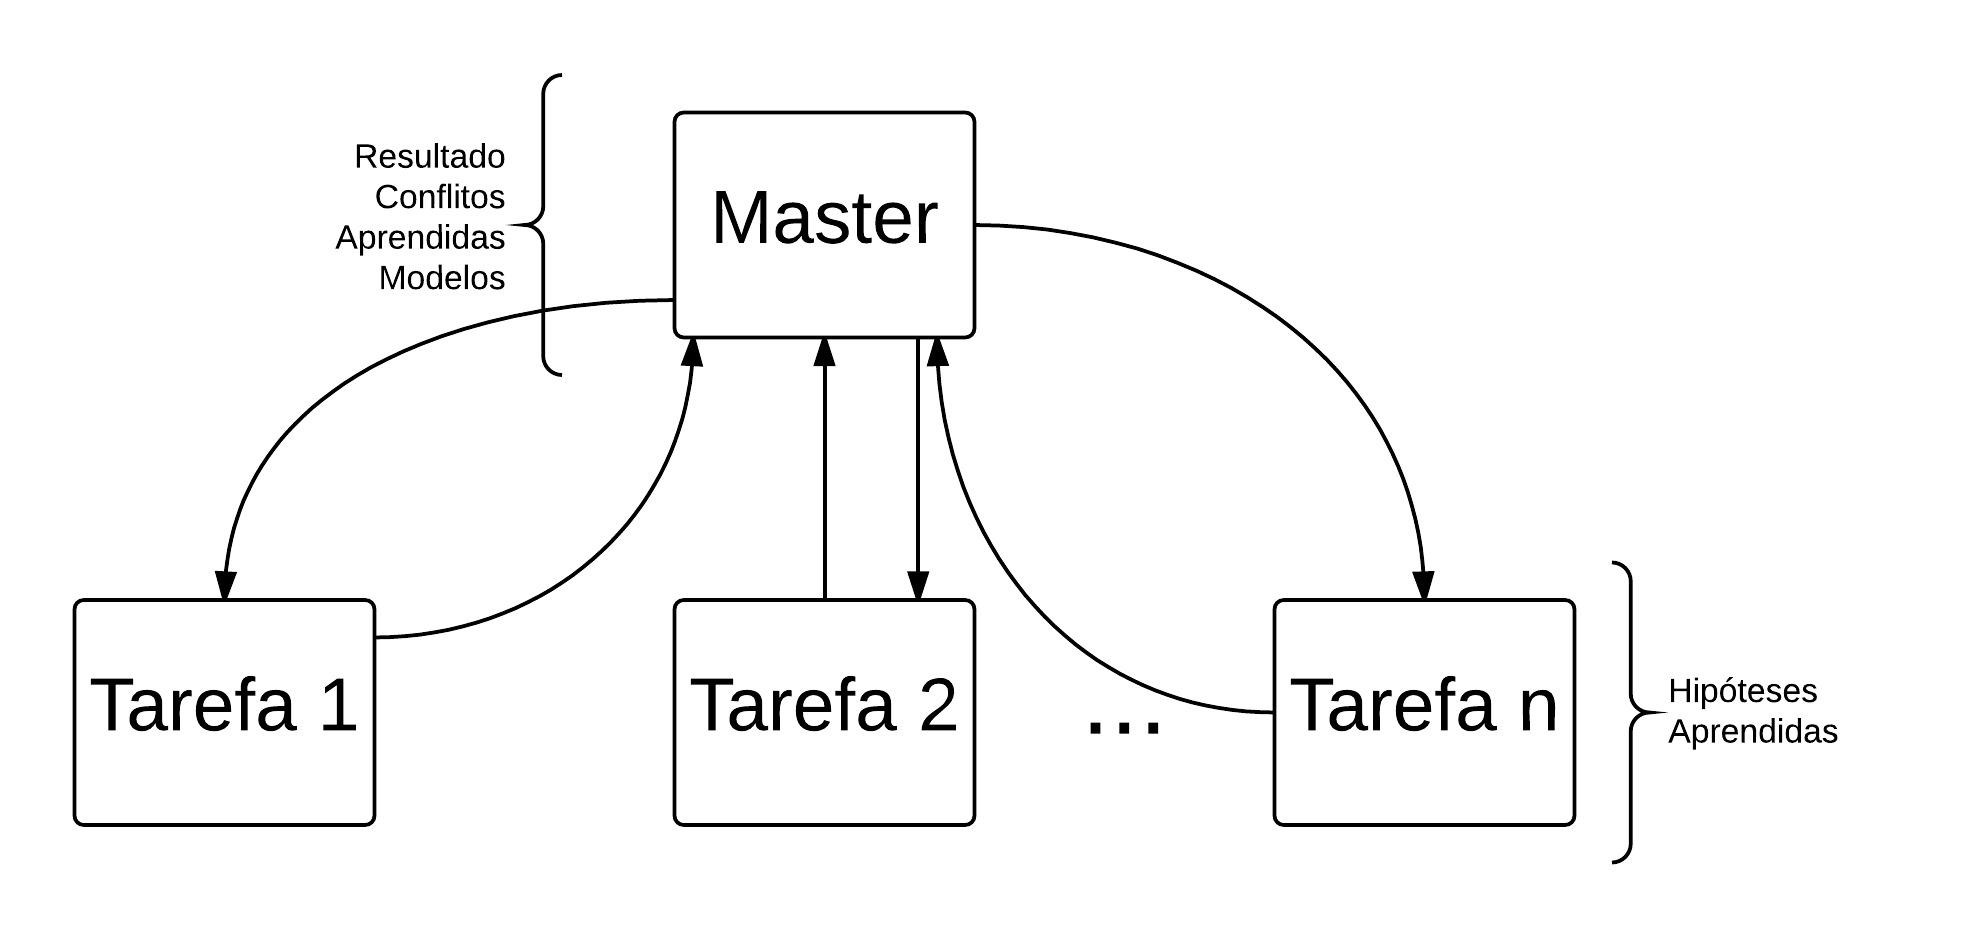
\includegraphics[width=0.8\textwidth]{figuras/PMSat.jpeg}
    \caption{Arquitetura do PMSat}
    \label{fig:PMSat}
\end{figure}

%GriSAT

No contexto de técnicas de paralelização existe uma técnica conhecida como portfólio, essa 
técnica consiste em executar múltiplos algoritmos distintos para solução de um problema 
comum, no caso do SAT múltiplos \textit{SAT Solvers}. Nesta técnica os algoritmos a serem 
utilizados devem ser escolhidos de forma a maximizar a velocidade de execução no caso médio, 
procurando-se escolher algoritmos com propriedades distintas. Seu speedup não pode ser avaliado 
pela Lei de Amdahl, pois não consiste na paralelização de um algoritmo e sim em uma técnica de 
execução em paralelo. Uma descrição desta técnica é apresentada na 
figura \ref{fig:port}

\begin{figure}[H]
    \centering
    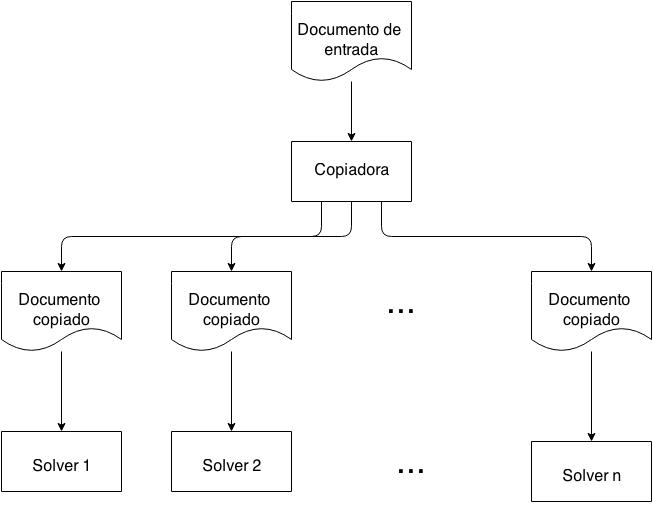
\includegraphics[width=0.8\textwidth]{figuras/portfolio.jpg}
    \caption{Funcionamento de um algoritmo portfólio\cite{nelson2013new}}
    \label{fig:port}
\end{figure}

Uma implementação popular da técnica portfólio para o problema SAT é o ManySAT\cite{Hamadi09manysat}. 
Este \textit{SAT solver} utiliza diferentes configurações aplicadas ao \textit{solver} 
MiniSAT e ao preprocessador SatElite, com isso ele obtém um bom ganho de desempenho 
pois os algoritmos baseados em DPLL modernos são bastante sensíveis as diferentes 
configurações de suas otimizações. O ManySAT foi amplamente testado em usos industriais 
de \textit{solver} e ficou em primeiro lugar do \textit{track} de paralelo da SAT-Race de 2008.
Este \textit{solver} foi desenvolvido pela Microsoft e pelo CRIL-CNRS.

Existem algoritmos \textit{SAT solvers} que são puramente estocásticos\allowbreak\cite{pprobSAT}
, por tanto sua execução não possui uma sequência de execução determinística. 
A paralelização destes algoritmos é trivial, sendo apenas necessário executar n 
instâncias do algorítimo, seu ganho é bom, seguindo a Lei de Amdahl o speedup 
teórico é de n.

\chapter{Desenvolvimento}

Nesta seção serão apresentados os diversos aspectos referentes ao desenvolvimento
do presente trabalho. Esta seção primeiro apresenta o algorítimo desenvolvido. Após são 
descritas as tecnologias utilizadas durante o desenvolvimento do trabalho, seu 
funcionamento e a motivação de sua escolha. Além disso também será apresentado o ambiente 
e metodologia de testes.

\section{Algoritmo de Busca}

Como dito anteriormente este algoritmo realiza uma busca em um espaço de estados. Esta busca 
é também a parte mais longa do algoritmo, uma vez que é necessário que a mesma visite todos os
estados possíveis do problema para que o mesmo seja provado insatifazivel ou para que sejam encontradas 
todas as soluções.

Existem dois modos de realizar uma busca em um espaço de estados, em largura(BFS) ou em profundidade(DFS). 
A busca em largura funciona partindo de uma raiz e visitando todos os seus vértices. A busca em profundidade 
funciona partindo de uma raiz e explorando cada ramo do espaço até que seja encontrado um nó folha, 
quando este é encontrado é realizado o backtracking.

Ambas as buscas pode ser exaustivas, assim visitando todos os nós possíveis, ou parar quando a primeira 
solução é encontrada. Sendo assim a implementação pode resolver tanto o problema SAT quanto suas 
extensões, como o USAT(UNIQUE-SAT). Para maioria dos casos é melhor parar na primeira solução encontrada, 
pois assim o algoritmo é mais rápido e raramente o tamanho da solução é importante.

TEMOS QUE VER ISSO
Para a implementação realizada neste trabalho utilizei a busca em profundidade, pois esta tende a achar 
uma solução para o problema antes.

Para a implementação deste trabalho utilizei a linguagem erlang, uma linguagem funcional, assim implementei 
uma versão recursiva do algoritmo de busca em profundidade. A versão clássica deste algorítimo funciona 
recebendo um grafo e um vértice a ser visitado. Marca-se o vértice como visitado e recursivamente chama-se 
a função para todos vértices adjacentes ainda não marcados como visitados. Esta versão pode ser vista no
pseudo código a seguir:

\begin{algorithm}
\caption{Pseudocódigo de um algoritmo funcional de busca em profundidade(DFS)} \label{alg:dfs}
\begin{algorithmic}[1]
\Procedure{DFS}{G,v}
\State marque v como visitado
\For{todo vértice w em G.verticesAdjacentes(v)}
  \If{w não é marcado como visitado}
    \State DFS(G,w)
  \EndIf
\EndFor
\EndProcedure
\end{algorithmic}
\end{algorithm}

Porém no caso deste trabalho o grafo de estados não está pronto no momento em que o algoritmo é chamado,
ele é construído no momento em que o estado é visitado em seus sucessores são calculados. Sendo assim 
foi necessário modificar o algoritmo clássico para o cenário do trabalho. Para isso foi modificada a 
entrada da função, nesta implementação a função recebe uma pilha de estados a visitar. A partir daí 
o algoritmo desempilha o primeiro estado, calcula os seus sucessores, empilha em ordem os estados 
sucessores e recursivamente chama a função até que a pilha esteja vazia. Esta implementação básica 
é apresentada no pseudo código a seguir:

\begin{algorithm}
\caption{Pseudocódigo de um algoritmo funcional DFS para grafo incompleto} \label{alg:dfs-incomplete}
\begin{algorithmic}[1]
\Procedure{Busca}{S}
\If{S é vazio}
\State \textbf{return}
\Else
  \State Estado = desempilhe(S)
  \State Succ = encontreSucessores(Estado)
  \State empilhe(Succ, S)
  \State Busca(S)
\EndIf
\EndProcedure
\end{algorithmic}
\end{algorithm}

Na versão implementada neste trabalho o estado é composto por um $\phi$ incompleto, que é a lista 
de quantum associados ao estado. Um forbidden, que é a lista quantum que não podem mais ser associados 
ao estado. E o gap, que o conjunto de clausulas que não contém um literal no $\phi$.

Outra característica da implementação deste trabalho é o calculo dos sucessores, que é feita utilizando 
uma função de qualidade. Esta função seleciona o quantum que cobre o maior numero de clausulas, como 
critério de desempate é selecionado o quantum cujo mirror cobre o maior numero de clausulas. O estado cujo 
gap é vazio deve ser colocado como uma solução e não deve ser adicionado nos sucessores. Também deve-se 
considerar como final o estado que não reduz o tamanho gap, este não deve ser adicionado aos sucessores 
nem as soluções.

Uma descrição visual do funcionamento do algoritmo é apresentada na imagem a seguir.

\begin{figure}[H]
    \centering
    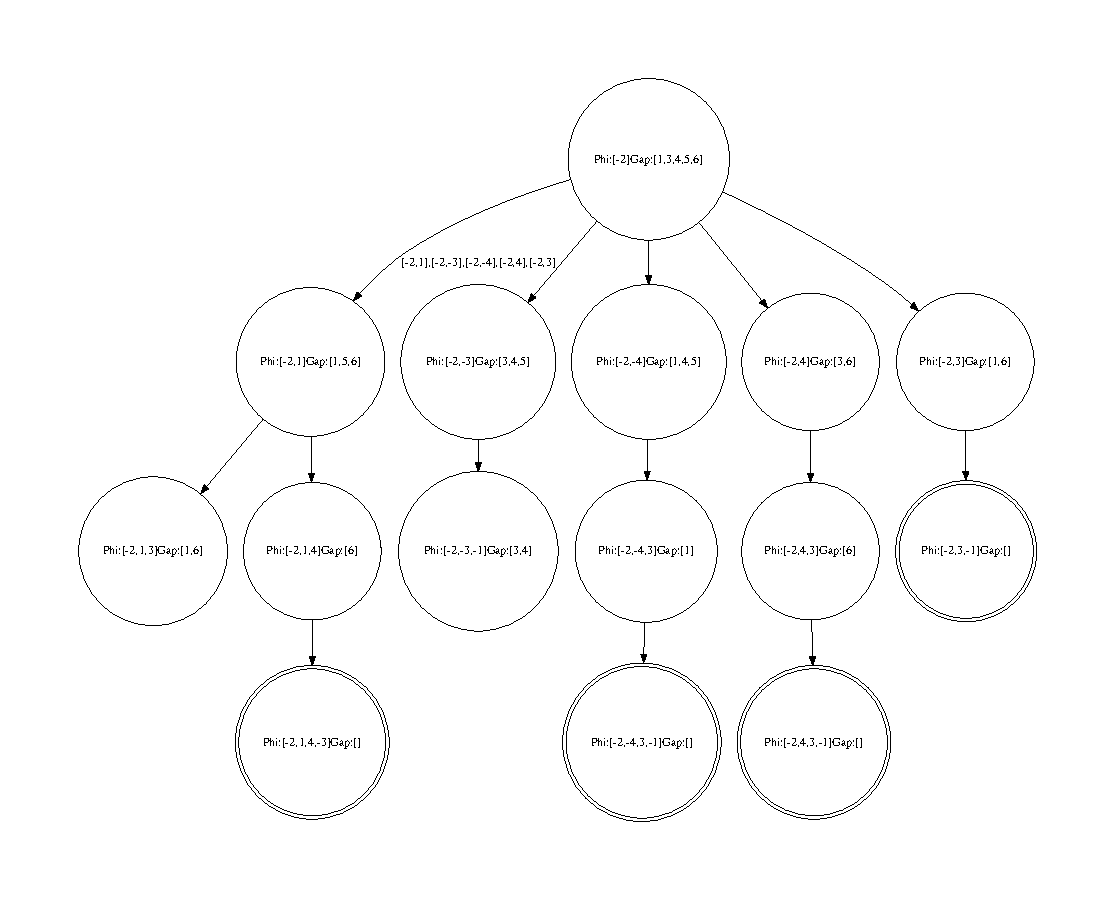
\includegraphics[width=1.2\textwidth]{figuras/AlgRep.pdf}
    \caption{Arvore de decisão da implementação do trabalho}
    \label{fig:AlgRep}
\end{figure}

\section{Busca Paralela}

Estudar como selecionar a busca utilizando a máquina da UFSC.

\bibliographystyle{abnt-num}
\bibliography{bibliografia}

\end{document}
